\section{Introduction}

%Multi-task learning is an inductive learning mechanism to improve generalization performance using related task data.
%Many state-of-the-art results in computer vision and natural language processing are obtained using multi-task learning.
Multi-task learning has recently become a powerful paradigm to solve complex prediction tasks in computer vision \cite{chexnet17,ZSSGM18}, natural language processing \cite{GLUE,superglue} and numerous other areas \cite{ZY17}.
%In multi-task learning, having related task data is fundamental to its performance.
%Multi-task learning is particularly powerful when there is limited labeled data for a task to be solved, meanwhile more labeled data from different but related tasks is available.
By combining multiple information sources, multi-task learning allows new information to be shared across different sources in a model \cite{C97}.
%For example, many applications in , and many other areas have been achieved by learning from multiple tasks together.
At the same time, it is well-known that the performance of multi-task learning methods depends on the relationship between the information sources.
\textit{Negative transfer}, the phenomenon where for a particular prediction task, multi-task learning performs worse than single-task learning, is prevalent when the information sources are heterogeneous \cite{AP16,BS17}.
While numerous studies have sought to alleviate negative transfer when it occurs \cite{YKGLHF20}, a rigorous understanding to the contributing causes of negative transfer has remained elusive in the literature \cite{R17}.
%This phenomenon, known as \textit{negative transfer}, is fundamental to the understanding of multi-task learning.
In this work, we consider learning multiple high-dimensional linear regression tasks to better understand when and why negative transfer happens. % for learning from multiple linear regression tasks.
We provide theoretical and practical insights to show how task data affects the transfer of information.
%We consider a setting where the target task has limited labeled data and show
%On the other hand, unless the structures across task data are well-understood, applying multi-task learning on several different datasets often result in suboptimal models (or negative transfer in more technical terms).

Identifying when negative transfer occurs requires comparing the performance of multi-task learning directly to single-task learning.
The technical challenge is to develop generalization bounds that are able to scale tightly with the qualities of task data, such as the number of datapoints.
In classical Rademacher or VC based theory of multi-task learning \cite{B00,AZ05,M06}, the generalization bounds are usually presented in a way so that the error goes down as more labeled data is added.
On the other hand, we have observed that adding more labeled data does not always improve performance in multi-task learning.
More recent work has shown the benefit of learning multi-task representations for certain half-spaces \cite{MPR16} and multipl sparse regressions \cite{LPTV09,LPVT11}.


%The technical challenge to develop a theory for multi-task learning is how to capture generalization performance that scales tightly with the amount of labeled data, in particular when the size of the training set is small.
%Prior generalization theory using uniform stability \cite{LTSM16}, Rademacher complexity \cite{BS03,BBCKP10} is unable to explain the phenomenon of negative transfer because there is no tight bound on test error that scales with the amount of labeled data.
%In particular in Figure \ref{fig_motivation}, we observe a shift from positive transfer to negative transfer as a parameter of task relatedness.
%The theory we develop will provide a precise explanation to such a phenomenon.

%To gain insight into the working of multi-task learning, we consider a simplified setting for learning multiple high-dimensional linear regression tasks.
%A typical process to do multi-task learning involves two steps:
%(i) Jointly learn a shared representation for all the tasks;
%(ii) Fine-tune the learnt model on a specific target task.
%We focus on a hard parameter sharing model proposed in \cite{R17,WZR20} and identify conditions on when multi-task and transfer learning works, and when it doesn't.
%The high-dimensional linear regression setting where the target task data size is limited captures the intuition that the target task only contains limited labeled data.

In this work, we consider multiple high-dimensional linear regression tasks as input and focus on predicting a particular task that only has limited amount of labeled data.
Following \cite{HMRT19,BLLT20}, we assume that for every task $1\le i\le t$, its features are random vectors $x = \Sigma_i^{1/2}z$, where $z\in\real^p$ consists of i.i.d. entries with mean zero and unit variance, and $\Sigma_i\in\real^{p\times p}$ is a positive semidefinite matrix.
The label of $x$ is given by $y_i = x^{\top}\beta_i + \varepsilon$, where $\beta_i\in\real^p$ denotes the ground truth parameters for task $i$ and $\varepsilon$ denotes random noise with mean zero and variance $\sigma^2$.
Importantly, we assume that for the target task $t$, its training data size $n_t$ is a small constant $\rho_t$ times $p$. %\todo{rational}
%We shall assume that each task data follows a linear model, i.e. $y_i = X_i \beta_i + \varepsilon_i$, $1\le i\le k$.
%Here $\beta_i\in\real^p$ is the model parameter for the $i$-th task.
%Each row of $X_i\in\real^{n_i\times p}$ is assumed to be drawn i.i.d. from a fixed
%distribution with covariance matrix $\Sigma_i$.
We use a hard parameter sharing architecture that contains a shared body $B\in\real^{p\times r}$ for all tasks and a separate prediction head $\set{W_i \in \real^{r}}_{i=1}^t$ for each task \cite{R17,MTDNN19}.
%    \paragraph{Different covariates:}
This corresponds to minimizing the following objective.
\begin{align}
	\label{eq_mtl}
	f(B; W_1, \dots, W_t) = \sum_{i=1}^t \norm{X_i B W_i - Y_i}^2.
\end{align}
%Note that we consider the natural parameterization without reweighting the tasks above.
%The shared body $B$ plays an important role because it allows information transfer between different task data.
%This is known as the hard parameter sharing architecture in the literature, where we control the capacity $r$ of $B$, e.g. \cite{KD12,WZR20}.
%We focus on comparing the test performance on a particular task solved with equation \eqref{eq_mtl} to single-task learning.
%The details are described in Algorithm \ref{alg_estimator}.
Let $\hat{\beta}_t^{\MTL} = B W_t$ denote the optimal predictor obtained from solving equation \eqref{eq_mtl} for task $t$.
Our goal is to compare the test error of $\hat{\beta}_t^{\MTL}$, denoted as $\te(\hat{\beta}_t^{\MTL})$, to $\te(\hat{\beta}_t^{\STL})$, where $\hat{\beta}_t^{\STL}$ is likewise obtained from equation \eqref{eq_mtl} but with task $t$ in isolation.


%\begin{figure}[!t]
%	\centering
%	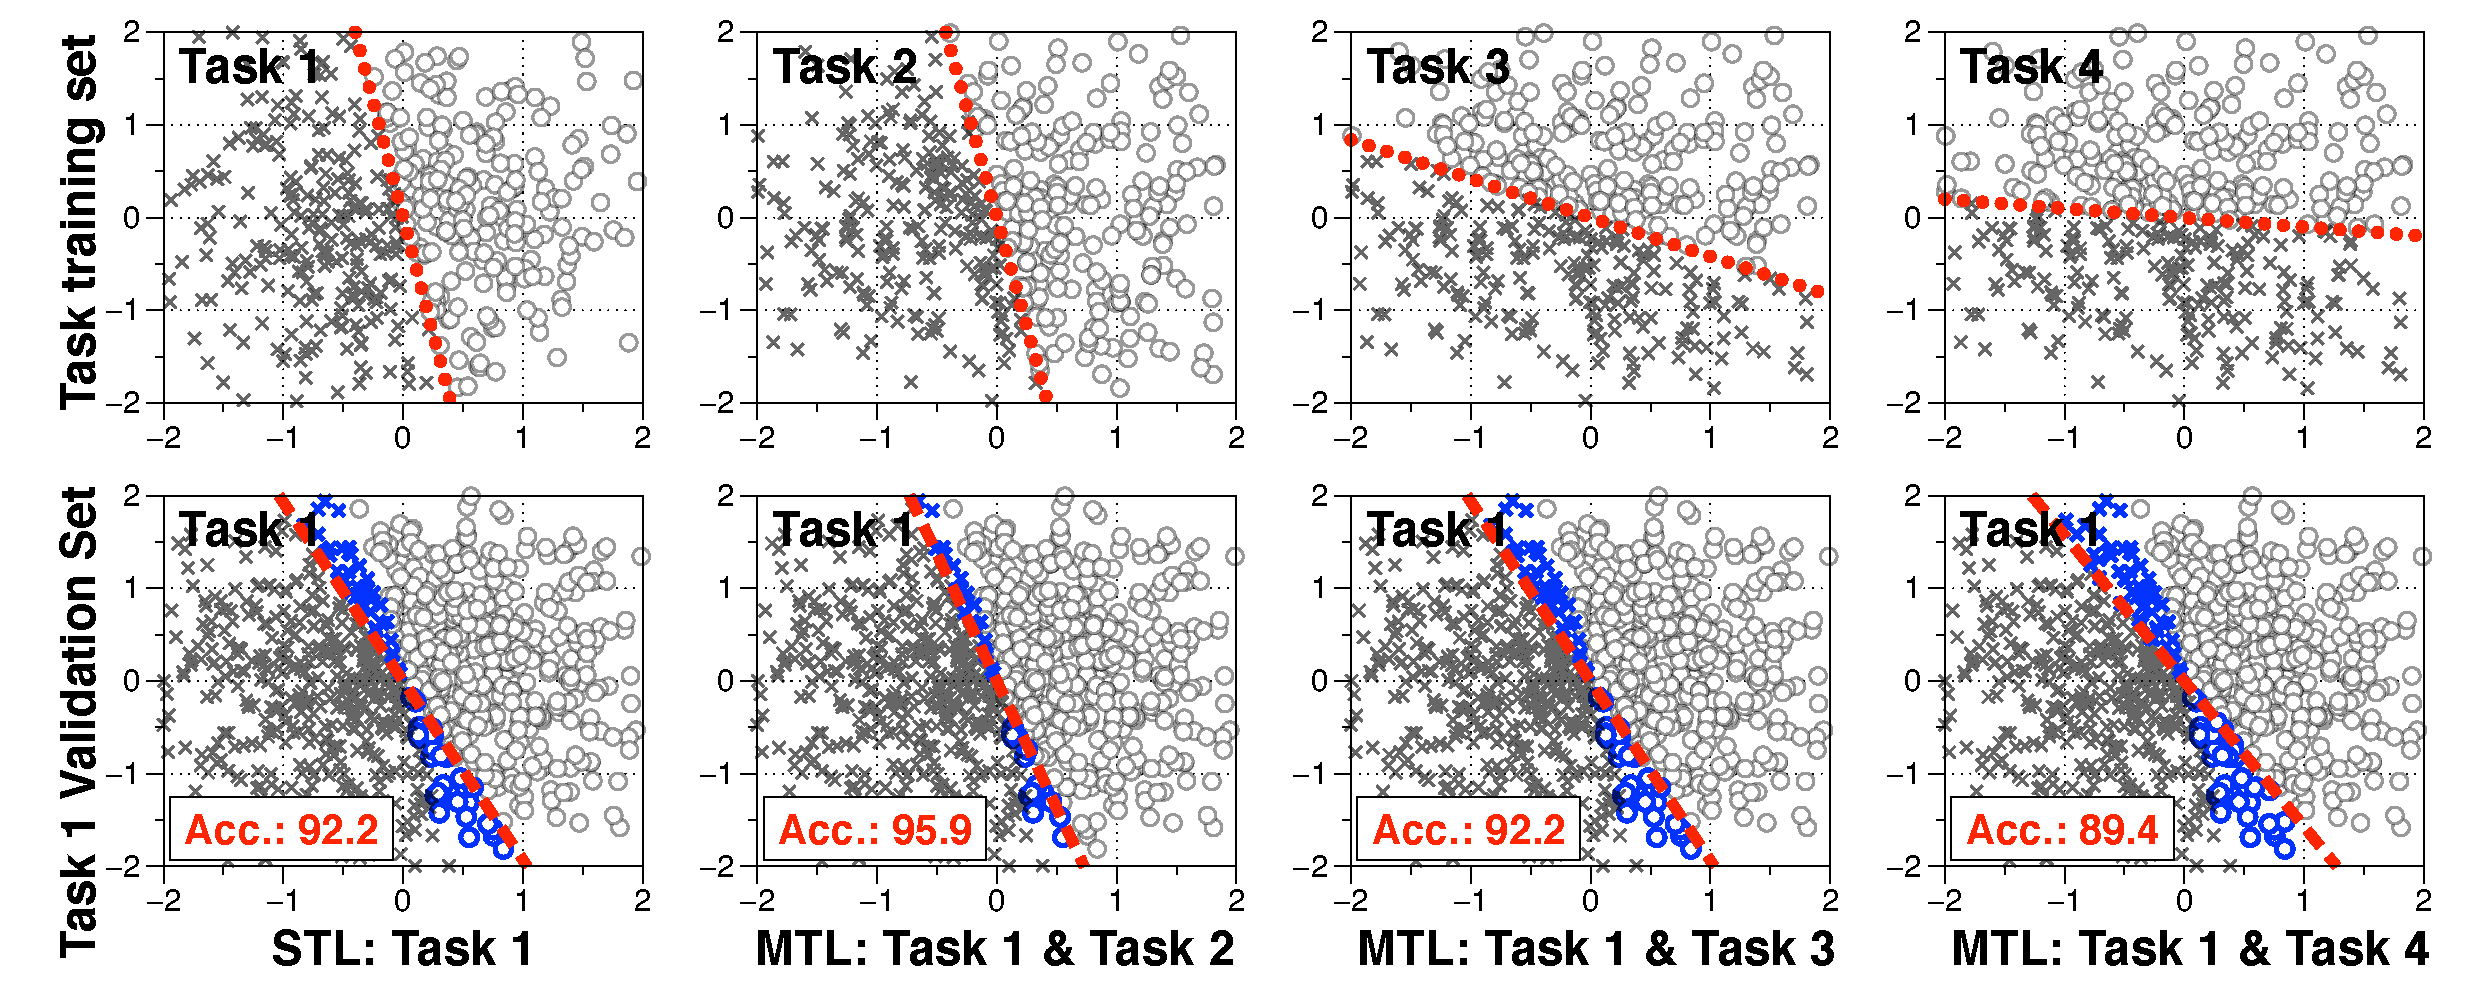
\includegraphics[width=0.8\textwidth]{figures/model_distance_motivation.pdf}
%	\caption{Positive to negative transfer as the source task rotates further away from the target task (left to right).}
%	\label{fig_motivation}
%\end{figure}


%We formulate the heterogeneity between different task data under covariate and model shifts .
%\begin{algorithm}[!t]
%	\caption{Multi-task learning using a hard-parameter sharing architecture}
%	\label{alg_estimator}
%	\begin{algorithmic}[1]
%		\Input Two regression tasks $(X_1, Y_2)$, $(X_2, Y_2)$.
%		\Param Shared body $B$, task-specific prediction heads $W_1, W_2$.
%		\State Training the shared body $B$.
%		\State Optimizing the task heads on the validation set

%		\begin{itemize}
%			\item Jointly optimizing both tasks: $\hat{\beta}_t^{\MTL}$
%			\item Optimizing the target task: $\hat{\beta}_t^{\TL}$
%			\item Single-task training baseline: $\hat{\beta}_t^{\STL}$
%		\end{itemize}
%		\State Problem statement: how can we compare the test error of the three estimators on the target task?
		%, $\te(\hat{\beta}_t^{\MTL})$, $\te(\hat{\beta}_t^{\STL})$ and $\te(\hat{\beta}_t^{\TL})$?
%	\end{algorithmic}
%\end{algorithm}

	\textbf{Main results.}
	We begin by observing that $\te(\hat{\beta}_t^{\MTL})$ can be decomposed into two parts, a variance part that is reduced from $\te(\hat{\beta}_t^{\STL})$, and a bias part that captures the difference between $\beta_t$ and the rest of $\beta$'s.
	We term the bias part as \textit{model shift bias}.
	Intuitively, whether $\te(\hat{\beta}_t^{\MTL})$ is lower than $\te(\hat{\beta}_t^{\STL})$ depends on the trade-off between the amount of variance reduced and the model shift bias part.
	For the high-dimensional regime when $p$ goes to infinity, we derive the asymptotic limit of $\te(\hat{\beta}_t^{\MTL}) - \te(\hat{\beta}_t^{\STL})$ as a function of the number of datapoints $\set{n_1, n_2}$, the covariance matrices $\set{\Sigma_1, \Sigma_2}$, the ground truth parameters $\set{\beta_1, \beta_2}$, and a certain fixed value derived from solving equation \eqref{eq_mtl} (see Theorem \ref{thm_main_informal} for the statement).
	Then, we show a similar result for any number of tasks that have the same covariates, i.e. the $X_i$'s are equal to each other.
	This setting is prevalent in applications of multi-task learning to image classification, where there are multiple prediction labels/tasks for every image \cite{chexnet17,EA20}.
	Based on the technical result, we provide theoretical insights over when multi-task learning performs better than single-task learning.

	Our first theoretical insight is to explain a sharp transition from positive to negative transfer as a parameter of \textit{task model dissimilarity} $\norm{\beta_1 - \beta_2}^2$.
	In Proposition \ref{prop_dist_transition}, we provide the trade-off between $\norm{\beta_1 - \beta_2}^2$ and a certain function $\Phi(\rho_1, \rho_2)$ to determine the type of transfer.

	Our second theoretical insight is to show that performing multi-task learning reduces the need for labeled data, which is a key finding of Taskonomy \cite{ZSSGM18}.
	We define \textit{data efficiency ratio} can be defined as the smallest $\alpha\in(0, 1)$ such that if we only use an $\alpha$ fraction of labeled data, then the test error of $\hat{\beta}_t^{\MTL}$ matches that of the $\hat{\beta}_t^{\STL}$ on the entire set.
	In Proposition \ref{prop_data_efficiency}, we consider an example and show that the data efficiency ratio is $\alert{\frac {1}{2\rho_t}}$.

	Our third theoretical insight is that as the data size becomes more imbalanced between the source and target task, having mis-aligned task covariance matrices can result in suboptimal performance.
	In Proposition \ref{prop_covariate}, we show that as $n_1 / n_2$ becomes large, the best performing source task has have the same covariance matrix as the target task.
	On the other hand, when $n_1 / n_2$ is small, there are counter examples where having the same covariance matrix is not necessarily the optimal choice.


Finally, while our focus is multi-task learning, our setup and technical tools are also applicable to transfer learning settings.
In Section \ref{sec_taskonomy}, we provide a case study of the transfer function used in Taskonomy \cite{ZSSGM18}.
We observe a similar trade-off between model-shift bias and variance for this setting.

A crucial technical tool that we develop for showing Theorem \ref{thm_main_informal} is the asymptotic limit of the trace of $(X_1^{\top}X_1 + X_2^{\top}X_2)^{-1}$ (for the setting of two tasks), which may be of independent interest.
The result extends a well-known result on the trace of $(X_1^{\top}X_1)^{-1}$ \cite{S07}
Furthermore, the error bound for the asymptotic limit is nearly optimal.

\textbf{Experimental results.} We show practical implications of our theoretical insights on text and image classification tasks.
	First, we provide a metric to determine positive versus negative transfer by comparing the test accuracies of single-task models.
	%validate on text and image classification tasks that comparing single-task accuracies can help determine whether multi-task learning performs better than single-task learning.
	Second, we validate that performing multi-task learning can reduce the need for labeled data.
	On 6 sentiment analysis tasks, we observe that just by using \alert{40\%} of the labeled data, the overall accuracy of multi-task learning matches that of learning every task in isolation.
	Finally, we show that as the data size between the source and target task becomes more imbalanced, aligning the covariances of the tasks becomes more beneficial.
%	On the other hand, if the number of source task datapoints is comparable to the target task, aligning task covariances may hurt performance.


